\documentclass[a4paper,11pt]{book}
%\documentclass[a4paper,twoside,11pt,titlepage]{book}
\usepackage{listings}
\usepackage[utf8]{inputenc}
\usepackage[spanish]{babel}

\usepackage[
backend=biber,
style=alphabetic,
sorting=ynt
]{biblatex}

\addbibresource{bibliografia.bib}

% \usepackage[style=list, number=none]{glossary} %
%\usepackage{titlesec}
%\usepackage{pailatino}

\decimalpoint
\usepackage{dcolumn}
\newcolumntype{.}{D{.}{\esperiod}{-1}}
\makeatletter
\addto\shorthandsspanish{\let\esperiod\es@period@code}
\makeatother


%\usepackage[chapter]{algorithm}
\RequirePackage{verbatim}
%\RequirePackage[Glenn]{fncychap}
\usepackage{fancyhdr}
\usepackage{graphicx}
\usepackage{afterpage}

\usepackage{longtable}

\usepackage[hidelinks]{hyperref}
\usepackage{glossaries}

\makeglossaries

\newglossaryentry{Malware}
{
    name=Malware,
    description={O software "malicioso" es todo aquél programa o código que pretende (de forma intencionada) causar daños y/o sacar beneficios de un sistema}
}

\newglossaryentry{cloud}
{
    name=Cloud,
    description={La computación en la nube o \textit{cloud} (del inglés cloud computing), conocida también como servicios en la nube, informática en la nube, nube de cómputo o simplemente «la nube», es un paradigma que permite ofrecer servicios de computación a través de una red, que usualmente es internet.}
}

\newglossaryentry{Ransomware}
{
    name=Ransomware,
    description={Es un tipo de malware que pretende hacer públicos o inaccesibles (por medio de encriptación, por ejemplo) los datos de la víctima hasta que esta pague un "rescate".}
}


\newglossaryentry{Reverse engineering}
{
    name={ingeniería inversa},
    description={Es una técnica que consiste en intentar obtener información sobre cómo está hecho o cómo funciona un producto a partir del propio producto en si. Intentando adivinar cómo funciona por medio de su uso y de pruebas que corroboren las suposiciones que se hagan.}
}

\newglossaryentry{obfuscation}{
    name={obfuscation},
    description={Ofuscación, ocultación, anonimato. Es el acto de evitar ser descubierto mientras realizas un ataque o una auditoría. Bien eliminando los rastros que puedas dejar u ocultándolos por medio de falsos rastros que escondan los tuyos.}
}

\newglossaryentry{network sniffing}
{
    name=network sniffing,
    description={Es la acción de "atender" al tráfico indiscriminado que circula por una red como si se fueran todos los posibles destinatarios con el objetivo de obtener una información que no fuera destinada a nosotros}
}

\newglossaryentry{Rolling Release}
{
    name=network sniffing,
    description={Es un tipo de distribución de Software en el que las actualizaciones son continuas en lugar de depender de un versionado discreto. Los cambios se van añadiendo de forma incremental conforme van siendo disponibles en lugar de ir emitiendo nuevas versiones con todos los cambios desde la anterior.}
}

\newglossaryentry{compilance}
{
    name=compilance,
    description={'el cumplimiento' de las normativas o leyes referentes a la seguridad de los datos que una empresa pueda almacenar o gestionar}
}

\newglossaryentry{vagrant}
{
    name=Vagrant,
    description={'una herramienta diseñada para el despliegue y configuración de entornos de máquinas virtuales (utilizando diversos proveedores como virtualbox, qemu, aws, etc...}
}

\newacronym{ddos}{DDOS}{Distributed Denial Of Service}

\newacronym{aws}{AWS}{Amazon Web Service}


\newacronym{iot}{IOT}{The Internet of Things}

\newglossaryentry{OpenSource}
{
    name=OpenSource,
    description={OpenSource o código abierto es un tipo de software liberado con una licencia que asegura el derecho de los usuarios a usar, estudiar, cambiar y distribuir el mismo con cualquier propósito.}
}

\newglossaryentry{Pull Request}
{
    name=OpenSource,
    description={Una Pull Request es la acción de validar un código que se va a mergear de una rama a otra. Por ejemplo, de una rama de desarrollo en un Fork de un proyecto a una rama oficial.}
}

\newacronym{IaC}{IAC}{Infrastructure as Code}
\newacronym{CPA}{CPA}{Certified Public Accountant}




% ********************************************************************
% Re-usable information
% ********************************************************************
\newcommand{\myTitle}{Integración de los procesos de Hacking ético en la plataforma de ciberseguridad de Wazuh \xspace}
\newcommand{\myDegree}{Grado en ingeniería informáticaxspace}
\newcommand{\myName}{Francisco Navarro Morales\xspace}
\newcommand{\myProf}{Alberto Guillén Perales\xspace}
%\newcommand{\mySupervisor}{Put name here\xspace}
\newcommand{\myFaculty}{Escuela Técnica Superior de Ingenierías Informática y de
Telecomunicación\xspace}
\newcommand{\myFacultyShort}{E.T.S. de Ingenierías Informática y de
Telecomunicación\xspace}
\newcommand{\myDepartment}{Departamento de ...\xspace}
\newcommand{\myUni}{\protect{Universidad de Granada}\xspace}
\newcommand{\myLocation}{Granada\xspace}
\newcommand{\myTime}{\today\xspace}
\newcommand{\myVersion}{Version 0.1\xspace}


%\hyphenation{}


%\usepackage{doxygen/doxygen}
%\usepackage{pdfpages}
\usepackage{url}
\usepackage{colortbl,longtable}
\usepackage[stable]{footmisc}
%\usepackage{index}

%\makeindex
%\usepackage[style=long, cols=2,border=plain,toc=true,number=none]{glossary}
% \makeglossary

% Definición de comandos que me son tiles:
%\renewcommand{\indexname}{Índice alfabético}
%\renewcommand{\glossaryname}{Glosario}

\pagestyle{fancy}
\fancyhf{}
\fancyhead[LO]{\leftmark}
\fancyhead[RE]{\rightmark}
\fancyhead[RO,LE]{\textbf{\thepage}}
\renewcommand{\chaptermark}[1]{\markboth{\textbf{#1}}{}}
\renewcommand{\sectionmark}[1]{\markright{\textbf{\thesection. #1}}}

\setlength{\headheight}{1.5\headheight}

\newcommand{\HRule}{\rule{\linewidth}{0.5mm}}
%Definimos los tipos teorema, ejemplo y definición podremos usar estos tipos
%simplemente poniendo \begin{teorema} \end{teorema} ...
\newtheorem{teorema}{Teorema}[chapter]
\newtheorem{ejemplo}{Ejemplo}[chapter]
\newtheorem{definicion}{Definición}[chapter]

\definecolor{gray97}{gray}{.97}
\definecolor{gray75}{gray}{.75}
\definecolor{gray45}{gray}{.45}
\definecolor{gray30}{gray}{.94}

\lstset{ frame=Ltb,
     framerule=0.5pt,
     aboveskip=0.5cm,
     framextopmargin=3pt,
     framexbottommargin=3pt,
     framexleftmargin=0.1cm,
     framesep=0pt,
     rulesep=.4pt,
     backgroundcolor=\color{gray97},
     rulesepcolor=\color{black},
     %
     stringstyle=\ttfamily,
     showstringspaces = false,
     basicstyle=\scriptsize\ttfamily,
     commentstyle=\color{gray45},
     keywordstyle=\bfseries,
     %
     numbers=left,
     numbersep=6pt,
     numberstyle=\tiny,
     numberfirstline = false,
     breaklines=true,
   }
 
% minimizar fragmentado de listados
\lstnewenvironment{listing}[1][]
   {\lstset{#1}\pagebreak[0]}{\pagebreak[0]}

\lstdefinestyle{CodigoC}
   {
	basicstyle=\scriptsize,
	frame=single,
	language=C,
	numbers=left
   }
\lstdefinestyle{CodigoC++}
   {
	basicstyle=\small,
	frame=single,
	backgroundcolor=\color{gray30},
	language=C++,
	numbers=left
   }

 
\lstdefinestyle{Consola}
   {basicstyle=\scriptsize\bf\ttfamily,
    backgroundcolor=\color{gray30},
    frame=single,
    numbers=none
   }


\newcommand{\bigrule}{\titlerule[0.5mm]}


%Para conseguir que en las páginas en blanco no ponga cabeceras
\makeatletter
\def\clearpage{%
  \ifvmode
    \ifnum \@dbltopnum =\m@ne
      \ifdim \pagetotal <\topskip
        \hbox{}
      \fi
    \fi
  \fi
  \newpage
  \thispagestyle{empty}
  \write\m@ne{}
  \vbox{}
  \penalty -\@Mi
}
\makeatother

\usepackage{pdfpages}
\begin{document}
\begin{titlepage}
 
 
\newlength{\centeroffset}
\setlength{\centeroffset}{-0.5\oddsidemargin}
\addtolength{\centeroffset}{0.5\evensidemargin}
\thispagestyle{empty}

\noindent\hspace*{\centeroffset}\begin{minipage}{\textwidth}

\centering

\includegraphics[width=0.9\textwidth]{imagenes/logo_ugr.jpg}\\[1.4cm]

\textsc{ \Large TRABAJO FIN DE GRADO\\[0.2cm]}
\textsc{ INGENIERÍA INFORMÁTICA}\\[1cm]
% Upper part of the page
% 
% Title
{\Huge\bfseries Integración de los procesos de Hacking ético en la plataforma de ciberseguridad de Wazuh \\
}
\noindent\rule[-1ex]{\textwidth}{3pt}\\[3.5ex]
{\large\bfseries Análisis de las distintas herramientas y procedimientos de offensive security y su integración con el software de Wazuh, así como el diseño y creación de un laboratorio de pruebas para test de penetración}
\end{minipage}

\vspace{2.5cm}
\noindent\hspace*{\centeroffset}\begin{minipage}{\textwidth}
\centering

\textbf{Autor}\\ {Francisco Navarro Morales}\\[2.5ex]
\textbf{Director}\\
{Alberto Guillén Perales\\}

\includegraphics[width=0.3\textwidth]{imagenes/etsiit_logo.png}\\[0.1cm]
\textsc{Escuela Técnica Superior de Ingenierías Informática y de Telecomunicación}\\
\textsc{---}\\
Granada, Septiembre de 2020
\end{minipage}
%\addtolength{\textwidth}{\centeroffset}
%\vspace{\stretch{2}}
\end{titlepage}



\chapter*{}
%\thispagestyle{empty}
%\cleardoublepage

%\thispagestyle{empty}

\begin{titlepage}
 
 
\setlength{\centeroffset}{-0.5\oddsidemargin}
\addtolength{\centeroffset}{0.5\evensidemargin}
\thispagestyle{empty}

\noindent\hspace*{\centeroffset}\begin{minipage}{\textwidth}

\centering
%
\includegraphics[width=0.9\textwidth]{imagenes/logo_ugr.jpg}\\[1.4cm]

%\textsc{ \Large PROYECTO FIN DE CARRERA\\[0.2cm]}
%\textsc{ INGENIERÍA EN INFORMÁTICA}\\[1cm]
% Upper part of the page
% 

 \vspace{3.3cm}

%si el proyecto tiene logo poner aquí

\includegraphics{imagenes/logo.png} 
 \vspace{0.5cm}

% Title

{\Huge\bfseries Título del proyecto\\
}
\noindent\rule[-1ex]{\textwidth}{3pt}\\[3.5ex]
{\large\bfseries Subtítulo del proyecto.\\[4cm]}
\end{minipage}

\vspace{2.5cm}
\noindent\hspace*{\centeroffset}\begin{minipage}{\textwidth}
\centering

\textbf{Autor}\\ {Nombre Apellido1 Apellido2 (alumno)}\\[2.5ex]
\textbf{Directores}\\
{Nombre Apellido1 Apellido2 (tutor1)\\
Nombre Apellido1 Apellido2 (tutor2)}\\[2cm]
%
\includegraphics[width=0.15\textwidth]{imagenes/tstc.png}\\[0.1cm]
%\textsc{Departamento de Teoría de la Señal, Telemática y Comunicaciones}\\
%\textsc{---}\\
%Granada, mes de 201
\end{minipage}
%\addtolength{\textwidth}{\centeroffset}
\vspace{\stretch{2}}

 
\end{titlepage}






\cleardoublepage
\thispagestyle{empty}

\begin{center}
{\large\bfseries Título del Proyecto: Subtítulo del proyecto}\\
\end{center}
\begin{center}
Nombre Apellido1 Apellido2 (alumno)\\
\end{center}

%\vspace{0.7cm}
\noindent{\textbf{Palabras clave}: palabra\_clave1, palabra\_clave2, palabra\_clave3, ......}\\

\vspace{0.7cm}
\noindent{\textbf{Resumen}}\\

Poner aquí el resumen.
\cleardoublepage


\thispagestyle{empty}


\begin{center}
{\large\bfseries Project Title: Project Subtitle}\\
\end{center}
\begin{center}
First name, Family name (student)\\
\end{center}

%\vspace{0.7cm}
\noindent{\textbf{Keywords}: Keyword1, Keyword2, Keyword3, ....}\\

\vspace{0.7cm}
\noindent{\textbf{Abstract}}\\

Write here the abstract in English.

\chapter*{}
\thispagestyle{empty}

\noindent\rule[-1ex]{\textwidth}{2pt}\\[4.5ex]

Yo, \textbf{Nombre Apellido1 Apellido2}, alumno de la titulación TITULACIÓN de la \textbf{Escuela Técnica Superior
de Ingenierías Informática y de Telecomunicación de la Universidad de Granada}, con DNI XXXXXXXXX, autorizo la
ubicación de la siguiente copia de mi Trabajo Fin de Grado en la biblioteca del centro para que pueda ser
consultada por las personas que lo deseen.

\vspace{6cm}

\noindent Fdo: Nombre Apellido1 Apellido2

\vspace{2cm}

\begin{flushright}
Granada a X de mes de 201 .
\end{flushright}


\chapter*{}
\thispagestyle{empty}

\noindent\rule[-1ex]{\textwidth}{2pt}\\[4.5ex]

D. \textbf{Nombre Apellido1 Apellido2 (tutor1)}, Profesor del Área de XXXX del Departamento YYYY de la Universidad de Granada.

\vspace{0.5cm}

D. \textbf{Nombre Apellido1 Apellido2 (tutor2)}, Profesor del Área de XXXX del Departamento YYYY de la Universidad de Granada.


\vspace{0.5cm}

\textbf{Informan:}

\vspace{0.5cm}

Que el presente trabajo, titulado \textit{\textbf{Título del proyecto, Subtítulo del proyecto}},
ha sido realizado bajo su supervisión por \textbf{Nombre Apellido1 Apellido2 (alumno)}, y autorizamos la defensa de dicho trabajo ante el tribunal
que corresponda.

\vspace{0.5cm}

Y para que conste, expiden y firman el presente informe en Granada a X de mes de 201 .

\vspace{1cm}

\textbf{Los directores:}

\vspace{5cm}

\noindent \textbf{Nombre Apellido1 Apellido2 (tutor1) \ \ \ \ \ Nombre Apellido1 Apellido2 (tutor2)}

\chapter*{Agradecimientos}
\thispagestyle{empty}

       \vspace{1cm}


Poner aquí agradecimientos...


%\frontmatter
%\tableofcontents
%\listoffigures
%\listoftables
%
%\mainmatter
%\setlength{\parskip}{5pt}
\printglossaries
\chapter{Introducción}

\section{\textit{Hacking} ético y seguridad ofensiva}

En un contexto marcado por el explosivo crecimiento de las tecnologías de la información, nuestras vidas se encuentran cada vez más ligadas a los dispositivos electrónicos y a sus posibles vulnerabilidades: el comercio electrónico y la banca \textit{online}, el uso correo electrónico como alternativa al tradicional, así como la creciente expansión del internet de las cosas (\textit{IOT}) en nuestras vidas o la enorme presencia de los dispositivos móviles en ella y el uso de la nube (\textit{Cloud Computing}), entre otros, crean un entorno en el que aquellos dispuestos a buscar y explotar las vulnerabilidades de nuestros sistemas pueden lucrarse y perjudicar gravemente a otros si no tomamos medidas.

    En este marco surgen constantemente más y más herramientas para asegurar la protección de nuestros dispositivos, tanto de los datos sensibles como de la disponibilidad de los mismos (ya sea porque un ataque inhabilite un servicio que ofrecemos o cierto tipo de \textit{Malware} nos impida acceder a nuestro dispositivo de forma regular). Entre todas estas herramientas surge \textbf{\textit{Wazuh}}, una plataforma \textit{OpenSource} de ciberseguridad que pretende convertirse en un estándar y una referencia a la hora de proteger nuestros sistemas y que engloba distintos tipos de módulos o herramientas que nos ofrecen, entre otras cosas, recolección y análisis de los registros (\textit{logs}) de nuestros \textit{endpoints}, detección de vulnerabilidades en el software instalado, control de la integridad de archivos sensibles o detección de intrusiones. 

Sin embargo, actualmente Wazuh se utiliza solo desde la perspectiva del administrador de sistemas que quiere asegurar la seguridad de su entorno desde dentro y no desde una perspectiva externa, la de un posible atacante intentando hallar un punto de acceso a su sistema. ¿Por qué podría interesarnos esto? Es aquí dónde entra en juego el Hacking ético y la seguridad ofensiva.

\subsection{Seguridad ofensiva}

Dicen que a veces la mejor defensa es un buen ataque. Pese a que las medidas que un administrador pueda tomar `desde dentro del sistema' pueden ser más que suficientes para proteger un dispositivo, cada vez están más presentes en el ámbito de la ciberseguridad aquellos que se ponen en la piel de un atacante e intentan encontrar puntos flacos en las defensas de un sistema \textbf{desde fuera}. Son los llamados \textbf{\textit{hacker éticos}}. Actuando dentro del marco legal y con permiso explícito de los dueños de un sistema, tratan de atacarlo como si fueran alguien intentando sacar algún provecho de estos o causar daños.

El mensaje ha calado con fuerza en la comunidad y diversos grupos de \textit{hackers} han desarrollado herramientas para lo que llaman "\textit{tests} de penetración de sistemas", en los que buscan extraer toda la información posible de un sistema por medio de técnicas como el escaneo de puertos, descifrado de contraseñas, análisis de redes (\textit{network sniffing}) o ingeniería inversa. 

Muchas de estas técnicas se pueden llevar a cabo por medio de herramientas OpenSource que suelen estar disponibles de un modo u otro en las distintas distribuciones de Linux. Es por ello que surgen diversas distribuciones especializadas en test de penetración como \textbf{Kali Linux} (basada en Debian) o \textit{Black Arch Linux}, un derivado de \textit{Arch Linux} con repositorios y herramientas pensadas para este tipo de tests.




\section{Estado del arte}

\section{Motivación}

\textit{Kali Linux} (así como otras distribuciones Linux orientadas a seguridad ofensiva) y la mayoría de sus herramientas son libres y gratuitas. Así como también lo es Wazuh. Dado que Wazuh pretende ofrecer a sus usuarios una \textbf{plataforma de ciberseguridad única} que reúna todo aquello que puedan necesitar para la seguridad de sus sistemas en único software (evitando así tener multitud de herramientas para cada necesidad distinta), sería interesante para ambas comunidades, la de Wazuh y la de hackers éticos que hacen uso de estas distribuciones, que se acortaran las distancias entre estas dos herramientas y se facilitara el uso conjunto de ambas. De esta forma, las dos herramientas podrían beneficiarse una de la otra y crear una comunidad conjunta sólida y robusta y el proyecto Wazuh (con sede en Granada) podría introducirse en la la escena de la ciberseguridad ofensiva basada en test de penetración.

\section{Justificación}

Wazuh consta de dos partes fundamentales: un \textit{agente}, que se instala en el \textit{endpoint} a monitorizar y recolecta información sensible para la seguridad del mismo, y un \textit{manager}, que recibe la información de distintos agentes y la procesa como eventos de interés que pueden (o no) generar alertas al usuario en función de la gravedad del evento.

Es decir, la principal utilidad de Wazuh no es proteger activamente tu sistema (como haría un antivirus) sino informar y dejar constancia de eventos críticos para la seguridad del mismo que hayan tenido lugar, para que podamos actuar en consecuencia.

Wazuh está diseñado para funcionar junto con \textit{Elasticsearch}, un motor de indexación que permite almacenar e indexar las alertas generadas por el manager para que sean fácilmente accesibles (por medio de consultas o a través de su interfaz gráfica, \textit{Kibana}, accesible a través de un navegador

\begin{figure}[hbt]
  \centering
    \reflectbox{%
      \includegraphics[width=0.5\textwidth]{example-image-a}}
  \caption{Ejemplo de visualización de alertas de seguridad indexadas en Elasticsearch por un manager Wazuh en el navegador usando Kibana}
\end{figure}

Por un lado, sería interesante poder realizar test de penetración sobre sistemas monitorizados por un agente \textit{Wazuh} y comprobar hasta qué punto este es capaz de detectar las intrusiones que se realicen desde el exterior y notificar o responder a eventos sensitivos.

Por otro lado, Wazuh podría servir a alguien sin acceso a un sistema a realizar un test de penetración sobre este analizando los logs de las distintas herramientas utilizadas durante el test y generando alertas según la relevancia de los eventos que se detectaran. Esto serviría para tener un registro de todo lo que se ha probado y los resultados obtenidos que podría servir como base para desarrollar un informe para una compañía para la que estuviéramos trabajando o simplemente para dejar constancia de los resultados obtenidos.

Así mismo, se podría aprovechar el potencial que ofrece el formato definido de alertas de Wazuh con Elasticsearch y Kibana para generar gráficas y \textit{dashboards} relacionados con los resultados del análisis. La propia base de datos de Elasticsearch, junto con su interfaz Kibana, podrían servir a modo de informe sobre un test realizado sobre varios sistemas.

Así pues, Wazuh es una herramienta potencialmente valiosa para estas distribuciones de Linux descritas. Potencial porque Wazuh utiliza un \textit{ruleset} con decodificadores de logs y reglas para generar alertas que, actualmente, no da soporte para la mayoría de herramientas de que disponen estos sistemas. Como hemos señalado, Wazuh está más orientado a buscar eventos sensibles en los logs de los servicios que correrían en un endpoint o en \textit{logs} de \textit{firewalls}, antivirus, etc... y no en la información que podría dar una herramienta de test de penetración.

Si realizamos una investigación de aquello que le falta a Wazuh para ser útil en este tipo de análisis, un posible desarrollo de decodificadores y reglas para esas herramientas podría suponer un paso enorme en el desarrollo del proyecto. Llevándolo a los administradores del mismo, es posible que estén dispuestos a integrarlo en su software e incluso, eventualmente, dar soporte oficial para aquellas funcionalidades que se desarrollaran a lo largo de este trabajo de fin de grado.


\section{Objetivos}

Así pues, este proyecto sería esencialmente un proyecto de investigación: recopilar y analizar información sobre las distintas herramientas que se utilizan en análisis de penetración de sistemas, comparar las distintas distribuciones especializadas que podrían integrar Wazuh en ellas y realizar pruebas con ellas para extraer conclusiones. A partir de dichas conclusiones, se desarrollarían las mencionadas reglas y decodificadores para integrar estas herramientas en Wazuh y hacer posible su análisis con este, y se crearía un entorno para hacer pruebas. A partir de dicho entorno se podrían ir re-adaptando y mejorando las reglas y decodificadores, extraer conclusiones y desarrollar, si fuera de utilidad, dashboards o gráficos en Kibana para las reglas generadas.

Sin embargo, teniendo en cuenta el número de horas asociado al proyecto y con la idea de "crear" software que pueda respaldar la labor de investigación más allá de la creación de reglas y decodificadores y los posibles gráficos y dashboard, sería interesante abordar el proyecto desde una perspectiva de "infraestructura como código" (\textit{IaC}), es decir, llevar a la práctica la implementación de automatizaciones para el despliegue y aprovisionamiento de todo lo que necesite el proyecto. Por ejemplo, si se plantea exportar una máquina virtual con todo preparado para el funcionamiento de Wazuh en Kali Linux, no nos limitaremos a hacer una OVA y compartirla junto con esta memoria, sino que automatizaremos el procedimiento de generación de dicha OVA, de forma que se pueda actualizar y compartir esta fácilmente cuando haya una actualización de Kali Linux o de Wazuh.

Del mismo modo, los entornos de pruebas que se utilizaran para testear las herramientas de análisis de penetración de sistemas serán desplegados y aprovisionados de forma automática y el procedimiento para ello quedará registrado y documentado y tendrá una licencia libre para que pueda usarse para otros propósitos.

Por último, una parte importante del trabajo será intentar hacer llegar el mismo a la comunidad OpenSource y de hacking ético. Se pretenderá presentar el proyecto a la empresa que desarrolla Wazuh por si estuvieran interesados en integrar todos los cambios que se hicieran en su software y dar soporte para las nuevas funcionalidades propuestas y se publicaría todo el material desarrollado durante el trabajo en alguna web pública y en GitHub para intentar que el proyecto alcanzara a gente dispuesta a probarlo y utilizarlo en la práctica.

En resumen, los objetivos de este trabajo serían:

\begin{description}
    \item [Investigación sobre herramientas de hacking] cuales son las más utilizadas y por qué, que información se puede conseguir con ellas, qué tipo de alertas podría generar el output de estas herramientas y que distribuciones de Linux las poseen. Clasificación de tales herramientas según su utilidad y la selección de varias de ellas por cada clase definida, que serán aquellas que integraremos con Wazuh. Realización de pruebas con las mismas en el entorno desarrollado \textbf{[30 horas]}
    \item [Investigación sobre distribuciones de ciberseguridad] cuales son las más utilizadas y por qué. Comparativa y selección de una o varias de ellas para integrarla con Wazuh. \textbf{[5 horas]}
    \item [Creación de imagen de testing:] que integre Wazuh y aquellas herramientas seleccionadas que no estén disponibles (si las hay) en la distribución. Dicha plataforma será una máquina virtual generada de forma automática y exportada como OVA y otros formatos disponibles. \textbf{[15 horas]}
    \item [Diseño de un entorno de pruebas] para test de penetración, y desarrollo del mismo usando tecnologías como Vagrant o Terraform, Docker, etc... crearemos una infraestructura fácilmente desplegable en local o en la nube  que integre sistemas con varios sistemas operativos y varios software típicos de servidores empresariales (bases de datos, servidores web, WordPress, Nginx, etc..) conectados entre sí y con distintos tipos de interfaz de red e IPs (públicas, privadas...), distintas distribuciones de puertos y software instalado. \textbf{[60 horas]}
    \item [Investigación y conclusiones] una vez desarrollado el entorno de pruebas y la imagen de Linux con Wazuh y cualquier dependencia, habría una extensa labor de probar en dicho entorno las herramientas seleccionadas en el primer punto, extraer conclusiones respecto a su uso y utilidad en un entorno que imita la realidad y la creación de sus reglas, decodificadores, dashboards, etc. Este es un punto aparte pero a medida que se vayan creando dichos elementos, deberán ir probándose y  esta tarea se retroalimentará con la siguiente buscando mejorar la integración con Wazuh y realizar un pequeño informe del aprendizaje extraído de este estudio. \textbf{[70+ horas]}
    \item [Reglas y decoders] desarrollar aquellas reglas y decodificadores necesarios para las herramientas seleccionadas, que se integren en Wazuh y generen alertas deseables, con toda la información posible y de interés para posibles usuarios y para el proyecto de Wazuh. \textbf{[50 horas]}
    \item [Desarrollo de un dashboard] para test de penetración en la app de Wazuh en Kibana, que incluya gráficas y tablas con información relevante según sea necesario. Idealmente, la app podría generar automáticamente un reporte del test realizado que sirviera como base para un informe de vulnerabilidades. \textbf{[50 horas]}
    \item [Protocolo de actuación] una vez se tenga algo de experiencia con las distintas herramientas y se hayan hecho pruebas en sistemas de variada índole, se podría llegar a definir e, incluso, automatizar un protocolo base para llevar a cabo un test de penetración. Obviamente, dichos test requerirán cierta supervisión humana y muchas veces irán guiados por la situación y lo que dicten la lógica y los conocimientos de la persona realizando el test; sin embargo, tener un esquema definido puede ser útil tanto desde un punto de vista académico como práctico. \textbf{[20 horas]}
    
\end{description}

\section{Security vs Compilance}

Cuando hablamos en términos de ciberseguridad necesitamos destacar el término \Gls{compilance}, que podría traducirse como 'el cumplimiento' de las normativas o leyes referentes a la seguridad de los datos que una empresa pueda almacenar o gestionar. Cualquier compañía con acceso a datos sensibles de sus clientes está obligada a asegurar unos mínimos requisitos de seguridad en sus entornos y ser capaz de demostrar que los cumple. \cite{phoenixnap}

\textit{Compilance} significa la capacidad que tiene una empresa de detallar su estado de seguridad de acuerdo a una serie de requisitos regulados en forma de legislación o regulaciones de la industria o simplemente en base a unos estándar creados a partir de buenas prácticas aceptadas por la comunidad.

Algunos ejemplos importantes de \textit{'compilances'}

\begin{description}
\item[HIPAA](Health Insurance Portability and Accountability Act) Se aplica a compañías del ámbito sanitario y regulariza cómo dichas compañías deben manejar y asegurar la seguridad de los datos médicos personales de sus pacientes. 

\item[PCI DSS] (Payment Card Industry Data Security Standard) Creado por algunas compañías de la industria de pago con tarjetas de crédito que quiso normalizar como se asegurar la integridad de la información financiera de sus clientes. Wazuh \cite{wazuh-pci} cuenta con herramientas para asegurar este \textit{compilance} asegurando (entre otros) la detección de \textit{rootkits} 

\item[SOC Reports] Se trata de unos reportes de control de sistemas y organizaciones verificable, llevado a cabo por una \acrfull{CPA} para asegurar el cumplimiento de las normativas de seguridad cuando la compañía maneja datos sensibles de sus clientes.

\end{description}

\section{Fases de una auditoría de ciberseguridad}

\subsection{Recopilación de información}

La primera fase de toda auditoría de ciberseguridad o test de penetración sería la recopilación de toda la información posible sobre los objetivos. Necesitamos llegar a conocer puntos de acceso al sistema (IPs de los distintos servidores, servicios utilizados por estos y abiertos a peticiones externas, websites, etc...), así como posible vulnerabilidades relacionadas con los usuarios del mismo (correos electrónicos que podrían ser hackeables, contraseñas inseguras o nombres de usuario que aparezcan en bases de datos de la deep web, etc...)

En un caso real, empezaríamos por investigar a la empresa a la que vamos a monitorizar y recopilar toda la información posible sobre sus sistemas y usuarios. Como el estudio se realizará sobre máquinas virtuales y no existe una empresa real a la que investigar, en nuestro caso la primera fase consistirá principalmente en recopilar información a partir de las IPs, conocidas (suponemos realizada la fase de descubrimiento de hosts) de las mismas. Es decir, empezaremos por un escaneo de puertos y descubriremos aquellos servicios reconocibles desde el exterior, también intentaremos obtener información de la versión del sistema operativo del host y de los distintos servicios que ofrece, e intentaremos sobrepasar los firewalls. 


\section{Aspectos legales del pentesting}

En primer lugar discutiremos los aspectos legales del trabajo de un hacker ético o pen-tester. Es importante tenerlos en cuenta para evitar problemas legales en un futuro y también una de las razones más importantes por las que se requiere un \textbf{entorno de pruebas seguro}.

\subsection{Introducción y aspectos generales}
\subsection{Leyes en Europa}
\subsection{Leyes en España}



\subsection{HoneyPots y ADS}
\chapter{Fase 1: Entornos de pruebas y aspectos legales del pentesting}
\section{Introducción}

Existen multitud en entornos de pruebas disponibles en internet para practicar los aspectos relacionados con el hacking ético. Una de las principales razones para esto es la posibilidad de meterse en problemas legales si se trata de practicar con entornos reales y equipos que no nos pertenecen. Estos aspectos se discutiran en un apartado posterior.


\subsection{Entornos de pruebas disponibles en internet}

\begin{enumerate}
    \item "TheCyberMentor" https://github.com/hmaverickadams/Beginner-Network-Pentesting
    \item "Hackthissite" https://www.hackthissite.org/
    \item "Metasploitable" https://sourceforge.net/projects/metasploitable/
    \item "Sliim pentest-env" https://github.com/Sliim/pentest-env
    \item "Sliim pentest-lab" https://github.com/Sliim/pentest-lab
\end{enumerate}
\subsubsection{Comparativa de varios entornos}
\subsection{Cursos interesantes sobre pentesting}
\begin{enumerate}
    \item Metasploit unleashed Metasploit Unleashed https://www.offensive-security.com/metasploit-unleashed/
    \item MITRE ATT\&CK https://attack.mitre.org/
    \item TheCyberMentor beginner curse https://github.com/hmaverickadams/Beginner-Network-Pentesting
\end{enumerate}


\section{Wazuh como una herramienta de loggin, monitorización y reporte durante nuestro análisis}

Uno de los aspectos claves de Wazuh que nos han llevado a plantearnos su viabilidad como una herramienta de apoyo al test de penetración es su capacidad para analizar logs. Si se usa adecuadamente, Wazuh puede filtrar por nosotros logs de interés y generar alertas en tiempo real para eventos importantes que tengan lugar durante el análisis.

Por tanto, si decidimos monitorizar toda acción o comando ejecutado en un shell de nuestro entorno de pruebas (Kali Linux) con Wazuh, podremos registrar cada acción llevada a cabo durante los tests y reportar aquellas que sean de interés para quien lo necesite. Bien como una forma de compartir información entre los miembros de un equipo de pentesting (de forma similar a lo que haría el software \textbf{Fargate} o bien como una forma de reportar a nuestros clientes \textbf{qué hemos hecho durante el análisis} y \textbf{cómo lo hemos hecho}. Así, si hubiera algún problema en los sistemas testeados durante nuestra auditoría y alguien tratara de hacernos responsables de hecho tendríamos una baza muy importante en juego: un sistema que registra nuestras acciones y las reporta en tiempo real a algún responsable dentro de la empresa que nos contrata cualquier cosa que sea de su interés.

\section{Entorno de trabajo: Kali Linux y Wazuh}

Aunque una parte importante del entorno de pruebas son aquellas máquinas que vamos a tratar de atacar, la principal herramienta que usaremos en nuestro estudio será una imagen de Kali Linux a la que instalaremos un agente de Wazuh capaz de monitorizar el output de todos los comandos que nos interesen. 

Kali Linux es una \Gls{Rolling Release}, lo que significa que las actualizaciones se hacen de forma incremental y no tiene un versionado discreto. Para este estudio he utilizado una ISO etiquetada como \textbf{2020.03} y la he instalado en una máquina virtual limpia. A continuación, y siguiendo la guía oficial de Wazuh para la instalación en sistemas operativos basados en Debian, he instalado un agente de Wazuh en mi máquina virtual. He instalado la versión más reciente en este momento (3.13.1) aunque la intención es ir actualizándola conforme salgan nuevas versiones a lo largo del desarrollo del trabajo.

\begin{figure}[hbt]
  \centering
      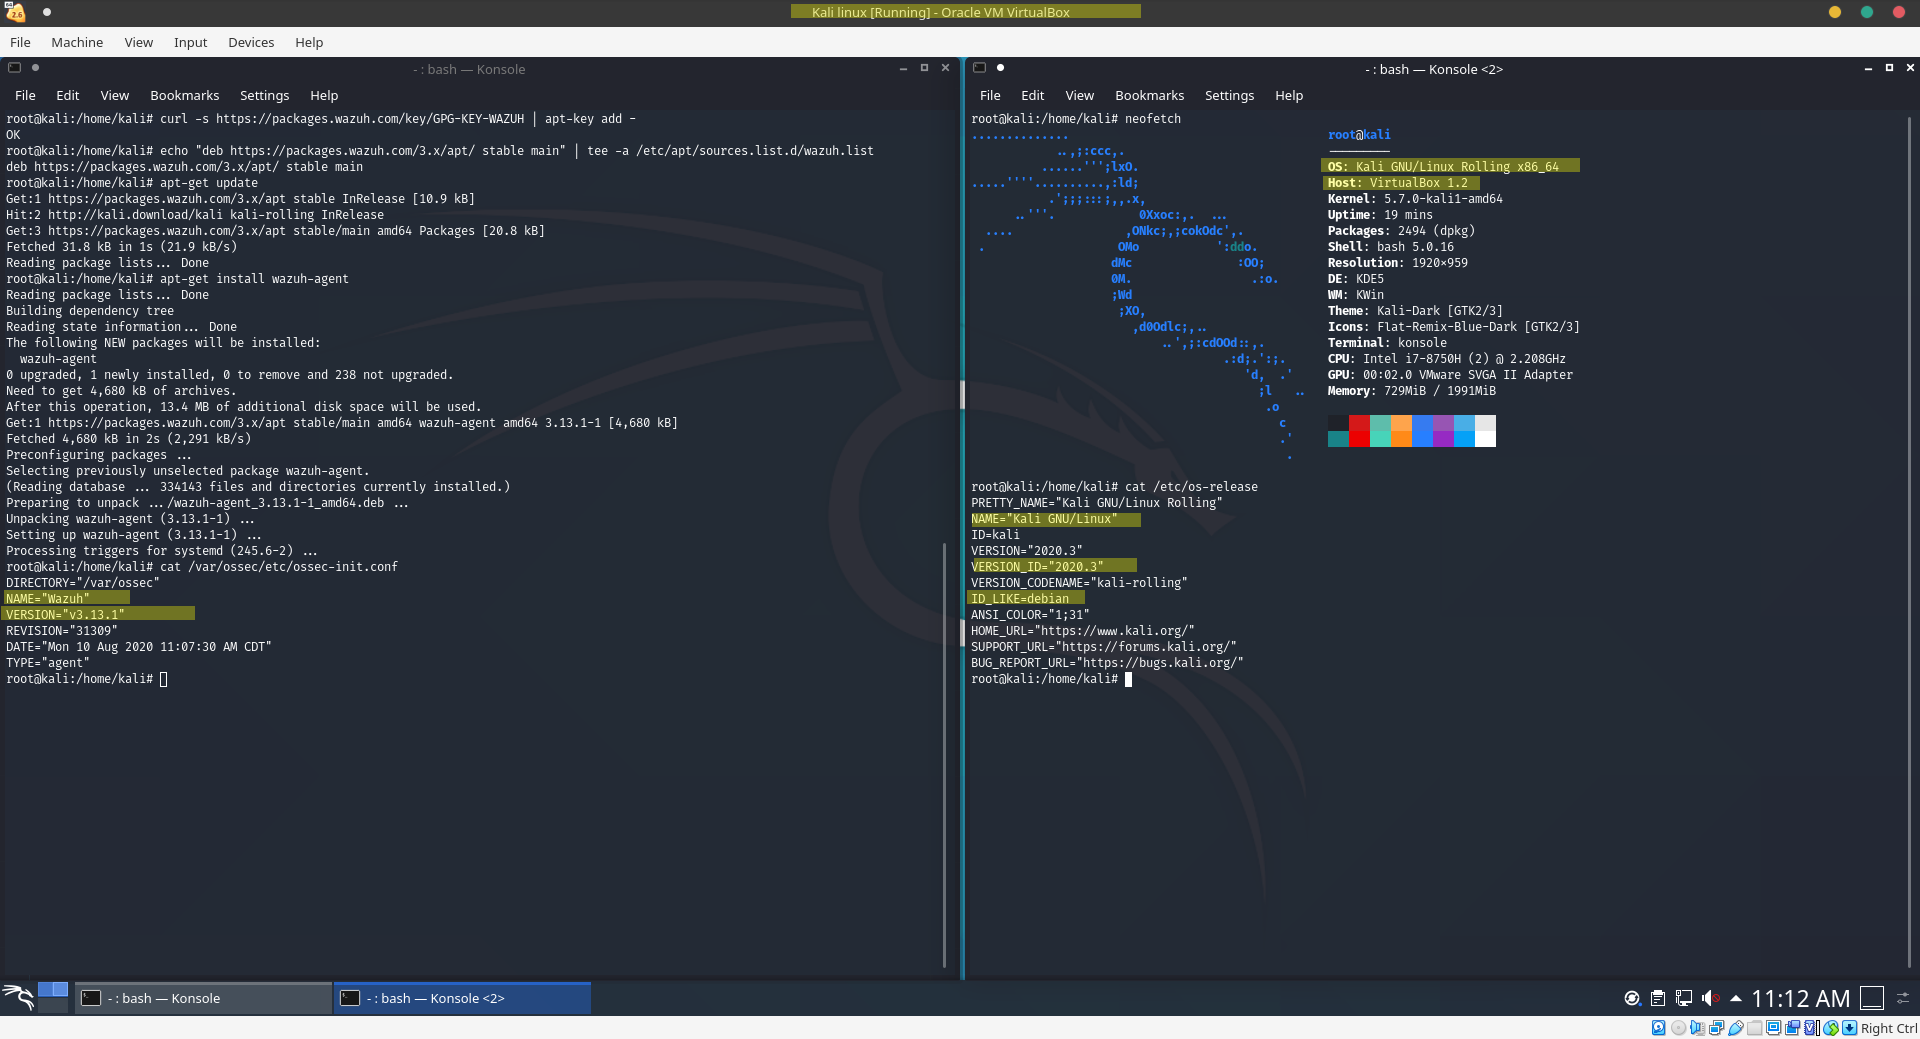
\includegraphics[width=\textwidth]{imagenes/kali_linux.png}
  \caption{Captura de pantalla del entorno virtualizado de Kali Linux mostrando alguna información del sistema y la instalación de Wazuh en varios terminales.}
\end{figure}

\section{}{Análisis de los resultados de las ejecuciones de los distintos comandos}
\subsection{Primera aproximación utilizando el comando script}

Para que Wazuh pueda generar alertas a partir del output de un comando ejecutado manualmente en un terminal, dicho output debe ser redirigido a un fichero que el agente pueda enviar al Manager para analizarlo. Para conseguir esto de forma sencilla he intentado utilizar la utilidad "script", un comando de Linux que nos permite registrar cada comando y su output en un fichero. Haciendo algunas modificaciones simples para que al iniciar una terminal interactiva el comando script se ejecute por defecto registrando los logs en un directorio concreto que será monitorizado por Wazuh y modificaremos la configuración por defecto del agente instalado en la instancia de Kali Linux para que solamente monitorice ese directorio.

El primer problema encontrado al utilizar \textit{script} para monitorizar todas las acciones llevadas a cabo durante una sesión es que este comando crea un entorno de trabajo (una shell) nuevo en cada ejecución del mismo, leyendo y ejecutando los archivos de configuración correspondientes al inicio de la misma. Esto se traduce en un bucle infinito si tratamos de comenzar una sesión de \textit{script} al inicio de una sesión bash, por ejemplo. Para solucionarlo, 

\begin{lstlisting}[language=bash,caption={Session recorder (/etc/profile)}]
if [ "x$SESSION_RECORD" = "x" ]
the
timestamp=$(date +%d-%m-%Y-%T)n
session_log=/var/log/session/session.$USER.$$.$timestamp
SESSION_RECORD=started
export SESSION_RECORD
script -t -f -q 2>${session_log}.timing $session_log
exit
fi

\end{lstlisting}

No obstante, esto no es suficiente. Script no nos permtie confiurar el formato del output que será enviado a Wazuh, y aunque podríamos usar herramientas extra para hacer este formateo, Script además escribe en el archivo de logs caracteres especiales de los terminales que sirven para codificar, entre otros, el color del texto, símbolos especiales, etc.. Por si fuera poco, Script guarda en sus logs el contenido tal y como aparecería en pantalla, lo que incluye lineas en blanco cuando se ejecuta un comando "clear", por ejemplo, y saltos de linea en el output de cada comando cuando este es muy largo.

Todo esto nos hace desechar esta opción y buscar una alternativa.

\subsection{Segunda aproximación usando "trampas" de Linux (comando trap)}

Una posible alternativa al comando script es utilizar las "trampas" (traps) de Linux, utilizando el comando \textbf{trap} podemos definir otro comando que se ejecutará antes de cualquier comando introducido en una shell. Así, podemos registrar el output de cada comando (así como el comando introducido en si) y calcular información como el nombre del usuario que lo ejecutó (\textbf{whoami}) o el timestamp del momento en que se ejecuta dicho comando. 

SOURCE: https://unix.stackexchange.com/questions/250713/modify-all-bash-commands-through-a-program-before-executing-them

\begin{lstlisting}[language=bash,caption={Session recorder (on bashrc file}]
shopt -s extdebug

preexec_invoke_exec () {
    [ -n "$COMP_LINE" ] && return  # do nothing if completing
    [ "$BASH_COMMAND" = "$PROMPT_COMMAND" ] && return # don't cause a preexec for $PROMPT_COMMAND
    local this_command=`HISTTIMEFORMAT= history 1 | sed -e "s/^[ ]*[0-9]*[ ]*//"`;

    # So that you don't get locked accidentally
    if [ "shopt -u extdebug" == "$this_command" ]; then
        return 0
    fi

    if [[ "${this_command}" =~ \S*=.* ]]; then
      this_command_output=""
      echo "$(date '+%Y-%m-%d %H:%M:%S') $(whoami)@$(pwd)# ${this_command}: $this_command_output"
      return 0
    fi

    this_command_output=$(eval "${this_command}" | tee /dev/tty)
    this_command_output=$(echo "${this_command_output}" | tr '\n' ' ')

    echo "$(date '+%Y-%m-%d %H:%M:%S') $(whoami)@$(pwd)# ${this_command}: $this_command_output"
    # Modify $this_command and then execute it
    return 1 # This prevent executing of original command
}
trap 'preexec_invoke_exec' DEBUG
\end{lstlisting}

problemas encontrados con el código original de stack overflow:
1) programas como vim neceitan que el output se redirija por pantalla antes de que finalice el comando -> solución, usar \textbf{tee |}
2) si defines variables dentro de la función, esas variables no se exportarán a la shell que llama a la función. -> solución, si el comando tiene el formato "palabra=loquesea" se permite su ejecución y se logea solo el input.
3) clear command shouldnt be logged because it will print white spaces
4) cd command should be regularly executed as well as other commands like 


\subsection{Wazuh Manager, Elasticsearch y Kibana app}
Para que el agente de Wazuh instalado en nuestra máquina con Kali Linux nos sea útil, este debe ser registrado en un Wazuh Manager, preferiblemente uno que esté conectado a un nodo de Elasticsearch y Kibana. Para simplificar todo el despliegue de dicha infraestructura (así como la actualización de la misma si fuera necesario) voy a utilizar el repositorio oficial de Docker de Wazuh. Utilizando la herramienta \textbf{Docker-Compose} desplegaré fácilmente un entorno con 
 


----- INCISO --- ¿Merece la pena un agente en kali conectado a un manager en vetetuasaber dónde? 
Por qué no usar un manager directamente en Kali? 
Y si quiero un entorno de pruebas distribuido para un equipo y quiero que todos compartan alertas? Puedo? 
Respuesta: como queremos que la empresa que contrata al auditor de seguridad pueda "controlar" lo que hace el equipo de auditoría, es interesante que cada usuario tenga un AGENTE instalado, y el manager/elasticsearch esté centralizado y sea común a cada agente y disponible por el contratante!

\section{Pasos para la creación de la imagen custom}
-install kali linux base
-install kde plasma desktop environment
-install terminator
-install docker and docker-compose
-set up logging system on all users
-install wazuh agent, remove all unused modules and connect it to the manager
-add crontab job to delete log files older than a week (for example)
-export image! 






\section{Primera iteración: Metasploitable 3}

En la primera iteración de este estudio utilizaremos una imagen llamada \textbf{Metasplotable 3} \cite{metasploitable3} para crear una máquina virtual vulnerable de forma rápida y sin complicaciones.

Se trata de una tercera versión de un proyecto creado con la intención de ser utilizado para entrenar en el ámbito del test de penetración y sabemos de antemano que el software instalado en sus imágenes las hace fácilmente vulnerables.

Metasploitable3 está diseñado utilizado \gls{vagrant}, una herramienta que nos permitirá desplegar máquinas virtuales (con el software de virtualización que deseemos) fácilmente.  Utilizaremos el archivo de configuración o Vagrantfile proporcionado en el repositorio de GitHub de \textbf{rapid7}, autor de esta herramienta y \textbf{Virtualbox} como software de virtualización.

Metasploitable3 contiene dos imágenes, una \textbf{Ubuntu 14.04} y otra \textbf{Windows server 2018}, las probaremos las dos en este orden y trataremos de ganar acceso a las mismas simulando un ataque o una auditoría de seguridad.









\chapter{Fase 2: Análisis de las herramientas para el test de penetración}

\section{Análisis de input/output utilizando Wazuh}

En primer lugar, he creado un decodificador de logs sencillo para simplemente extraer el input introducido por el usuario y su output. Para comandos más interesantes (como nmap), utilizaremos un decodificador específico que sea capaz de separar la distinta información relevante.


\begin{lstlisting}[language=XML, caption=Custom base decoder for command execution logger]
<decoder name="shell_log">
<program_name>shell_log</program_name>
</decoder>

<decoder name="shell_command">
<parent>shell_log</parent>
<regex># (\.*) -> (\.*)</regex>
<order>command, output</order>
</decoder>
\end{lstlisting}

Este decodificador, combinado con una regla que genere alertas de bajo nivel (3, que es el mínimo para que aparezcan en la interfaz de Wazuh) nos permite empezar a guardar información de todo lo que ocurra en el sistema.

\begin{lstlisting}[language=XML, caption=Custom base rule for command execution logger]
<group name="shell_execution">
  <rule id="66600" level="3">
  <decoded_as>shell_log</decoded_as>
  <description>$(command) executed. Output: $(output)</description>
</rule>
and, output</order>
</decoder>
\end{lstlisting}

No obstante, hay que tener cuidado con no llenar nuestros discos con información irrelevante o redundante. Por eso, cuando el proyecto esté más avanzado, modificaremos el nivel de las alertas basandose en el comando ejecutado, deforma que no guardemos la información de comandos como ls, top, pwd, cat, etc..

En las siguientes secciones describiremos algunas herramientas de interés en tests de penetración de sistemas así como las reglas y/o decodificadores desarrollados para las mismas.

\section{Distribuciones de Linux para pentesting}
\section{Clasificación de herramientas}
\subsection{Recopilación de información: descubrimiento de hosts y escaneo de puertos}
A la hora de detectar los hosts visibles dentro de una red y qué servicios ofrece (y son visibles) podemos encontrar diversas herramientas:

\begin{description}
    \item[ping] Commando simple que permite enviar ICMP "echo requests" a hosts en la red para ver si están en funcionamiento.
    \item [nmap] Herramienta de escaneo de redes que utiliza paquetes IP (raw) para determinar los hosts disponibles en una red y los servicios que ofrecen.
    \item [metasploit framework] : ) 
\end{description}
\section{Análisis de las distintas herramientas}

\subsection{Nmap}

Nmap es una herramienta muy versátil y que puede ofrecer muchísima información sobre los diferentes endpoints en una red (aunque puede analizar hosts individualmente, parte de su interés radica en que puede ser utilizada para analizar redes enteras). Permite detectar aquellos servidores con determinados puertos abiertos o aquellos puertos que tiene abiertos cada servidor, las versiones del sistema operativo del endpoint o de los servicios que ofrece e incluso muchas vulnerabilidades de los mismos. Además, tiene numerosas opciones que permiten modificar el tipo de comunicación que se hará durante el escaneo e incluso la velocidad del mismo (un escaneo muy rápido podría suponer problemas con el firewall) o tratar de anonimizar los paquetes enviados durante el escaneo para conseguir ocultar nuestras acciones (\Gls{obfuscation})  

Algunos ejemplos del uso de nmap que pueden ser de interés para el estudio y que podemos utilizar para empezar a desarrollar las reglas de Wazuh que generarán alertas cuando nmap detecte información relevante.

\begin{table}[!hbtp]
\begin{tabular}{|l|l|l|}
\hline
flags & example                    & usage                                      \\ \hline
      & nmap 172.1.1.0/24          & Default scan a network using CIDR notation \\ \hline
-sS   & nmap 172.1.1.11 -sS        & TCP SYN port scan (Default)                \\ \hline
-sT   & nmap 192.1.10.10 -sT       & TCP connect port scan                      \\ \hline
-sA   & nmap 122.122.1.1 -sA       & TCP ACK port scan                          \\ \hline
-p    & nmap 122.128.1.1 -p 21-100 & scan ports in a range                      \\ \hline
-O    & nmap -O 172.10.1.22        & OS detection                               \\ \hline
-Tn   & nmap 192.168.1.10 -T2      & n={0,1,..,5} regulates the scan speed      \\ \hline
\end{tabular}
\caption{Some examples of nmap usage}
\label{tab:my-table}
\end{table}


\input{capitulos/05_Test_Penetración}

%
%%\chapter{Conclusiones y Trabajos Futuros}
%
%
%%\nocite{*}

%\appendix
%\input{apendices/manual_usuario/manual_usuario}
%%\input{apendices/paper/paper}
%\input{glosario/entradas_glosario}
% \addcontentsline{toc}{chapter}{Glosario}
% \printglossary

\medskip

\printbibliography

\chapter*{}
\thispagestyle{empty}



\end{document}
